\begin{figure}[htb]
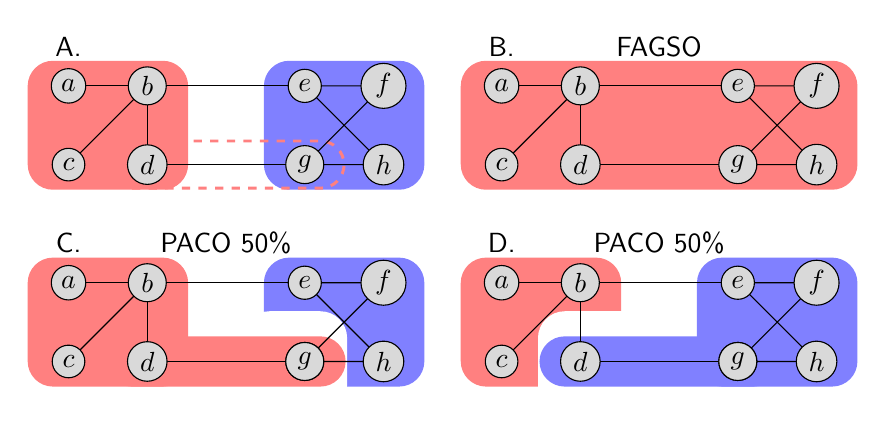
\begin{tikzpicture}
%\draw[help lines,step=1] (0,-5) grid (10,5);
\begin{scope}[shift={(0,0)}]
\fill [red!50, draw, rounded corners=2ex,line width=0.25ex] (-0.5,-0.3) rectangle (1.5,1.3);
\fill [blue!50, draw, rounded corners=2ex,line width=0.25ex] (2.5,-0.3) rectangle (4.5,1.3);
\draw [red!50, draw, rounded corners=2ex, dashed, line width=0.25ex] (0.5,-0.3) rectangle (3.5,0.3);
\draw (0,1) -- (1,1);
\draw (1,1) -- (1,0);
\draw (1,0) -- (1,1);
\draw (1,1) -- (0,0);
\draw (1,0) -- (3,0);
\draw (1,1) -- (3,1);
\node [fill=gray!30, radius=1ex, draw, circle, inner sep=2pt] at (0,1) {$a$};
\node [fill=gray!30, radius=1ex, draw, circle, inner sep=2pt] at (1,1) {$b$};
\node [fill=gray!30, radius=1ex, draw, circle, inner sep=2pt] at (0,0) {$c$};
\node [fill=gray!30, radius=1ex, draw, circle, inner sep=2pt] at (1,0) {$d$};
\draw (3,1) -- (4,1) -- (3,0) -- (4,0) -- cycle;
\node [fill=gray!30, radius=1ex, draw, circle, inner sep=2pt] at (3,1) {$e$};
\node [fill=gray!30, radius=1ex, draw, circle, inner sep=2pt] at (4,1) {$f$};
\node [fill=gray!30, radius=1ex, draw, circle, inner sep=2pt] at (3,0) {$g$};
\node [fill=gray!30, radius=1ex, draw, circle, inner sep=2pt] at (4,0) {$h$};
\node at (0,1.5) {\textsf{A.}};
\end{scope}

\begin{scope}[shift={(5.5,0)}]
\node at (2,1.5) {\textsf{FAGSO}};
\node at (0,1.5) {\textsf{B.}};
\fill [red!50, draw, rounded corners=2ex,line width=0.25ex] (-0.5,-0.3) rectangle (4.5,1.3);
\draw (0,1) -- (1,1);
\draw (1,1) -- (1,0);
\draw (1,0) -- (1,1);
\draw (1,1) -- (0,0);
\draw (1,0) -- (3,0);
\draw (1,1) -- (3,1);
\node [fill=gray!30, radius=1ex, draw, circle, inner sep=2pt] at (0,1) {$a$};
\node [fill=gray!30, radius=1ex, draw, circle, inner sep=2pt] at (1,1) {$b$};
\node [fill=gray!30, radius=1ex, draw, circle, inner sep=2pt] at (0,0) {$c$};
\node [fill=gray!30, radius=1ex, draw, circle, inner sep=2pt] at (1,0) {$d$};

\draw (3,1) -- (4,1) -- (3,0) -- (4,0) -- cycle;
\node [fill=gray!30, radius=1ex, draw, circle, inner sep=2pt] at (3,1) {$e$};
\node [fill=gray!30, radius=1ex, draw, circle, inner sep=2pt] at (4,1) {$f$};
\node [fill=gray!30, radius=1ex, draw, circle, inner sep=2pt] at (3,0) {$g$};
\node [fill=gray!30, radius=1ex, draw, circle, inner sep=2pt] at (4,0) {$h$};
\end{scope}

\begin{scope}[shift={(0,-2.5)}]
\node at (2,1.5) {\textsf{PACO 50\%}};
\node at (0,1.5) {\textsf{C.}};
\fill [red!50, draw, rounded corners=2ex,line width=0.25ex] (-0.5,-0.3) rectangle (1.5,1.3);
\fill [blue!50, draw, rounded corners=2ex,line width=0.25ex] (2.5,-0.3) rectangle (4.5,1.3);
\draw (1,1) -- (3,1);
\fill [white, draw, rounded corners=2ex, line width=0.5ex] (2.25,-0.6) rectangle (3.5,0.6);
\fill [red!50, draw, rounded corners=2ex, line width=0.25ex] (0.5,-0.3) rectangle (3.5,0.3);
\draw (1,0) -- (3,0);
\draw (3,1) -- (4,1) -- (3,0) -- (4,0) -- cycle;
\node [fill=gray!30, radius=1ex, draw, circle, inner sep=2pt] at (3,1) {$e$};
\node [fill=gray!30, radius=1ex, draw, circle, inner sep=2pt] at (4,1) {$f$};
\node [fill=gray!30, radius=1ex, draw, circle, inner sep=2pt] at (3,0) {$g$};
\node [fill=gray!30, radius=1ex, draw, circle, inner sep=2pt] at (3,0) {$g$};
\node [fill=gray!30, radius=1ex, draw, circle, inner sep=2pt] at (4,0) {$h$};
\draw (0,1) -- (1,1);
\draw (1,1) -- (1,0);
\draw (1,0) -- (1,1);
\draw (1,1) -- (0,0);
\node [fill=gray!30, radius=1ex, draw, circle, inner sep=2pt] at (0,1) {$a$};
\node [fill=gray!30, radius=1ex, draw, circle, inner sep=2pt] at (1,1) {$b$};
\node [fill=gray!30, radius=1ex, draw, circle, inner sep=2pt] at (0,0) {$c$};
\node [fill=gray!30, radius=1ex, draw, circle, inner sep=2pt] at (1,0) {$d$};
\end{scope}

\begin{scope}[shift={(5.5,-2.5)}]
\node at (2,1.5) {\textsf{PACO 50\%}};
\node at (0,1.5) {\textsf{D.}};
\fill [red!50, draw, rounded corners=2ex,line width=0.25ex] (-0.5,-0.3) rectangle (1.5,1.3);
\fill [blue!50, draw, rounded corners=2ex,line width=0.25ex] (2.5,-0.3) rectangle (4.5,1.3);
\draw (1,1) -- (3,1);
\fill [white, draw, rounded corners=2ex, line width=0.5ex] (0.5,-0.6) rectangle (2,0.6);
\fill [blue!50, draw, rounded corners=2ex, line width=0.25ex] (0.5,-0.3) rectangle (3.5,0.3);
\draw (1,0) -- (3,0);
\draw (3,1) -- (4,1) -- (3,0) -- (4,0) -- cycle;
\node [fill=gray!30, radius=1ex, draw, circle, inner sep=2pt] at (3,1) {$e$};
\node [fill=gray!30, radius=1ex, draw, circle, inner sep=2pt] at (4,1) {$f$};
\node [fill=gray!30, radius=1ex, draw, circle, inner sep=2pt] at (3,0) {$g$};
\node [fill=gray!30, radius=1ex, draw, circle, inner sep=2pt] at (3,0) {$g$};
\node [fill=gray!30, radius=1ex, draw, circle, inner sep=2pt] at (4,0) {$h$};
\draw (0,1) -- (1,1);
\draw (1,1) -- (1,0);
\draw (1,0) -- (1,1);
\draw (1,1) -- (0,0);
\node [fill=gray!30, radius=1ex, draw, circle, inner sep=2pt] at (0,1) {$a$};
\node [fill=gray!30, radius=1ex, draw, circle, inner sep=2pt] at (1,1) {$b$};
\node [fill=gray!30, radius=1ex, draw, circle, inner sep=2pt] at (0,0) {$c$};
\node [fill=gray!30, radius=1ex, draw, circle, inner sep=2pt] at (1,0) {$d$};
\end{scope}
\end{tikzpicture}
\caption{Difference in atomic operation between PACO and FAGSO algorithms. In A. both the algorithms consider the edge $d-g$. While FAGSO is merging communities as the result of every operation on edges, PACO is more 
If the operation of merging the red and blue communities in one leads to an increment in Surprise then for FAGSO the operation is carried and the algorithm continues. For PACO instead, nodes are moved with by chance in a community or in another, resulting in two different possible results. In this case the result in D. has higher Surprise than the result in C. but PACO may equally explore the solution C.}
\label{fig:pacofagso}
\end{figure}